This chapter covers the architecture and design of the system.
\section{General architecture}
In this section the general architecture of the THERESA system is described.
The idea for the new system is to reuse the concept of the already existing sampling system KAPTURE (\textbf{Ka}rlsruhe \textbf{P}ulse \textbf{T}aking \textbf{U}ltra-fast \textbf{R}eadout \textbf{E}lectronics), which is using four ADCs, and expanding it to 16. Therefore, also the architecture of the latter is explained briefly.
\subsection{KAPTURE-2}
KAPTURE, which was developed at IPE, is a system designed to continuously sample ultra-short pulses generated by Terahertz detectors. It consists of a daughter card, holding four sampling channels, mounted on a FPGA . The FPGA is connected to a computer via PCIe for further processing of the acquired data. \cite{brosi} 
The newer version, KAPTURE-2, was designed for more accurate sampling for pulse repetition rates up to \SI{2}{\giga \hertz}. The acquired data is processed with a FPGA and GPU architecture.  \cite{caselleKAP}

The general structure of the board is shown in \autoref{fig:kapture}.

\begin{figure}[H]
	\centering
	\includegraphics[width = \textwidth]{chap/03-work/img/kapture.tikz}
	\caption{General schema of KAPTURE-2 (cf. \cite[p.2]{caselleKAP})}
	\label{fig:kapture}
\end{figure}


The pulse from the \SI{}{\tera \hertz} detector is fed into a power splitter, which splits the signal into four identical pulses and distributes them to four channels, consisting of a respective Track-And-Hold-Amplifier (THA) unit and a 12-bit ADC@\SI{500}{\mega\sample\per\second}. The sampling time of each unit can be adjusted individually with a Picosecond Delay Chip with a resolution of \SI{3}{\pico \second} (maximal delay range: \SI{100}{\pico \second}). 
The clock signal is provided by KARA, which is cleared from jitter by a Phase-Locked-Loop (PLL). This ensures the synchronization of the ADCs with the RF system. The clean clock signal is distributed to the delay chips via fan-out. \cite{caselleKAP}

The resulting sampling of the detector signal is shown \autoref{fig:detector_signal} (simplified representation).
\begin{figure}[H]
	\centering
	\includegraphics[height = 0.3\textwidth, width = 0.6\textwidth]{chap/03-work/img/detector_signal.tikz}
	\caption{Signal with sample points}
	\label{fig:detector_signal}
\end{figure}

\begin{figure}[H]
	\centering
	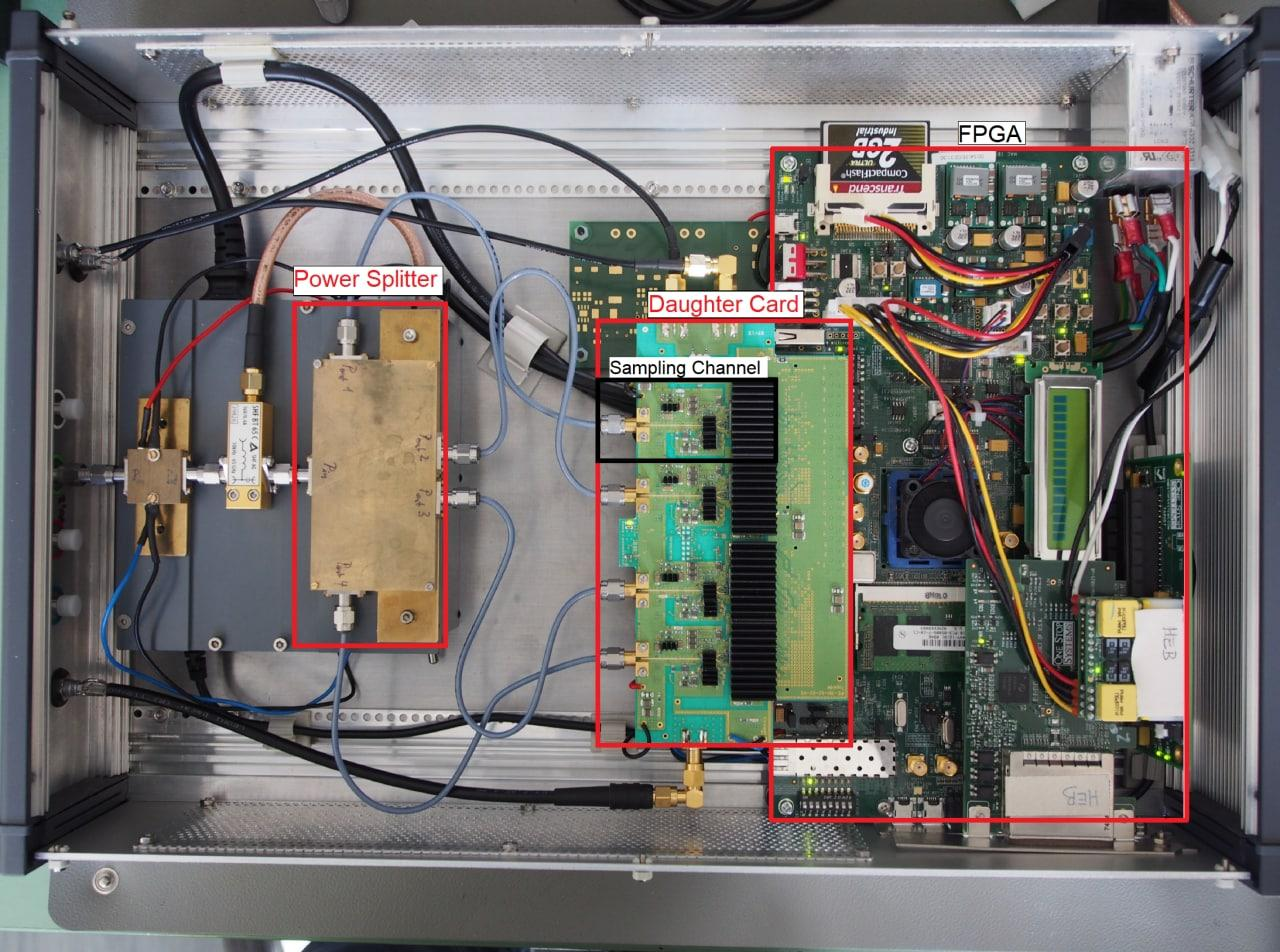
\includegraphics[width = 0.8\textwidth]{chap/03-work/img/kapture_sys}
	\caption{Photo of KAPTURE with highlighted main components. \cite[p.~61]{brosi}}
	\label{fig:kapturesys}
\end{figure}

\newpage
\subsection{New System THERESA}
In principle, the new system has the same structure, as KAPTURE. Notable differences are firstly the number of ADCs, which is increased up to 16. Secondly, the latter are not located on the daughter card anymore, but inside the Xilinx Zynq UltraScale+ RFSoC ZU49DR on the ZCU216 Evaluation Kit on which the front-end card is mounted. \autoref{fig:theresa_scheme} shows the general schema of the sampling system, reduced to four channels for presentation purposes.
\begin{figure}[H]
	\centering
	\includegraphics[width = \textwidth]{chap/03-work/img/theresa_scheme.tikz}
	\caption{General schema of THERESA. For presentation purposes only four channels are shown.}
	\label{fig:theresa_scheme}
\end{figure}

\paragraph{Xilinx Zynq UltraScale+ RFSoC ZCU216 Evaluation Card}
The card, holding the sampling channels, should be mounted on a ZCU216 evaluation board. This board is the newest generation of Xilinx' evaluation cards, which has features suitable for the purpose at hand.
\begin{itemize}[noitemsep]
\item Sixteen 14-bit, 2.5GSPS RF-ADC
\item Sixteen 14-bit, 10GSPS RF-DAC
\item I/O expansion options – FPGA Mezzanine Card (FMC+) interfaces, RFMC 2.0 interfaces, and Pmod connections
\end{itemize}
\begin{figure}[H]
	\centering
	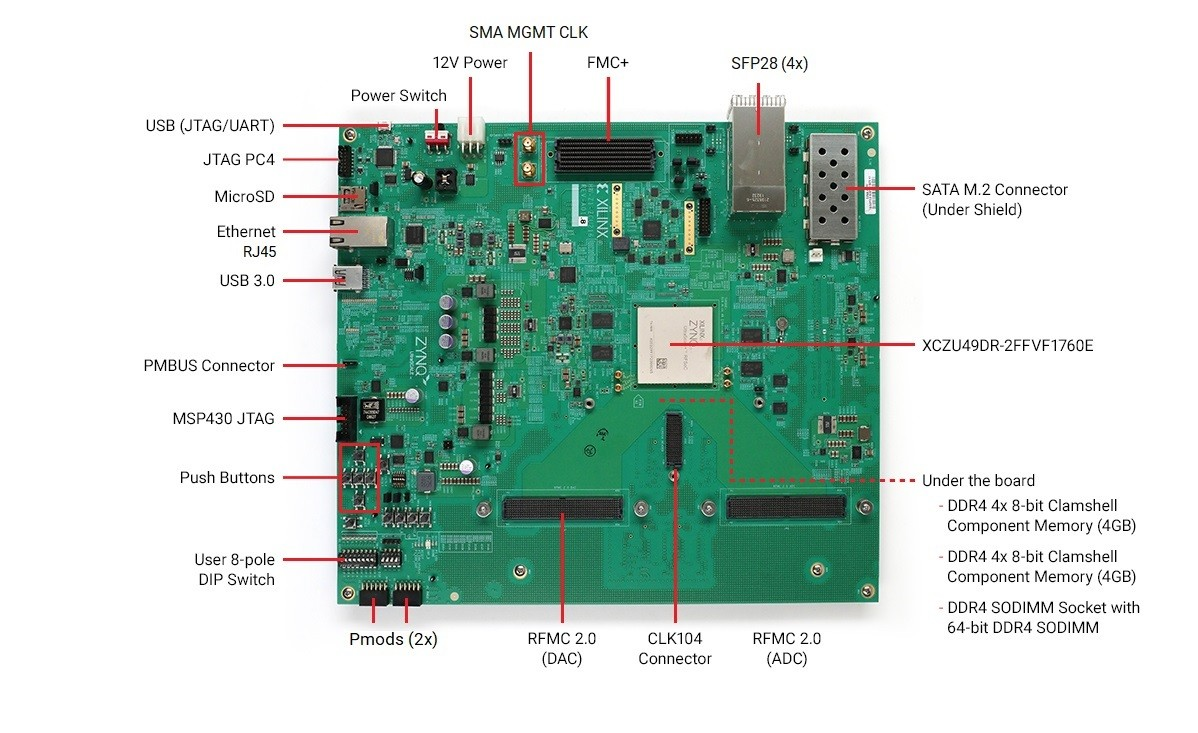
\includegraphics[width = \textwidth]{chap/03-work/img/zcu216}
	\caption{ZCU216 evaluation board}
	\label{fig:zcu216}
\end{figure}
 
\begin{figure}[H]
	\centering
	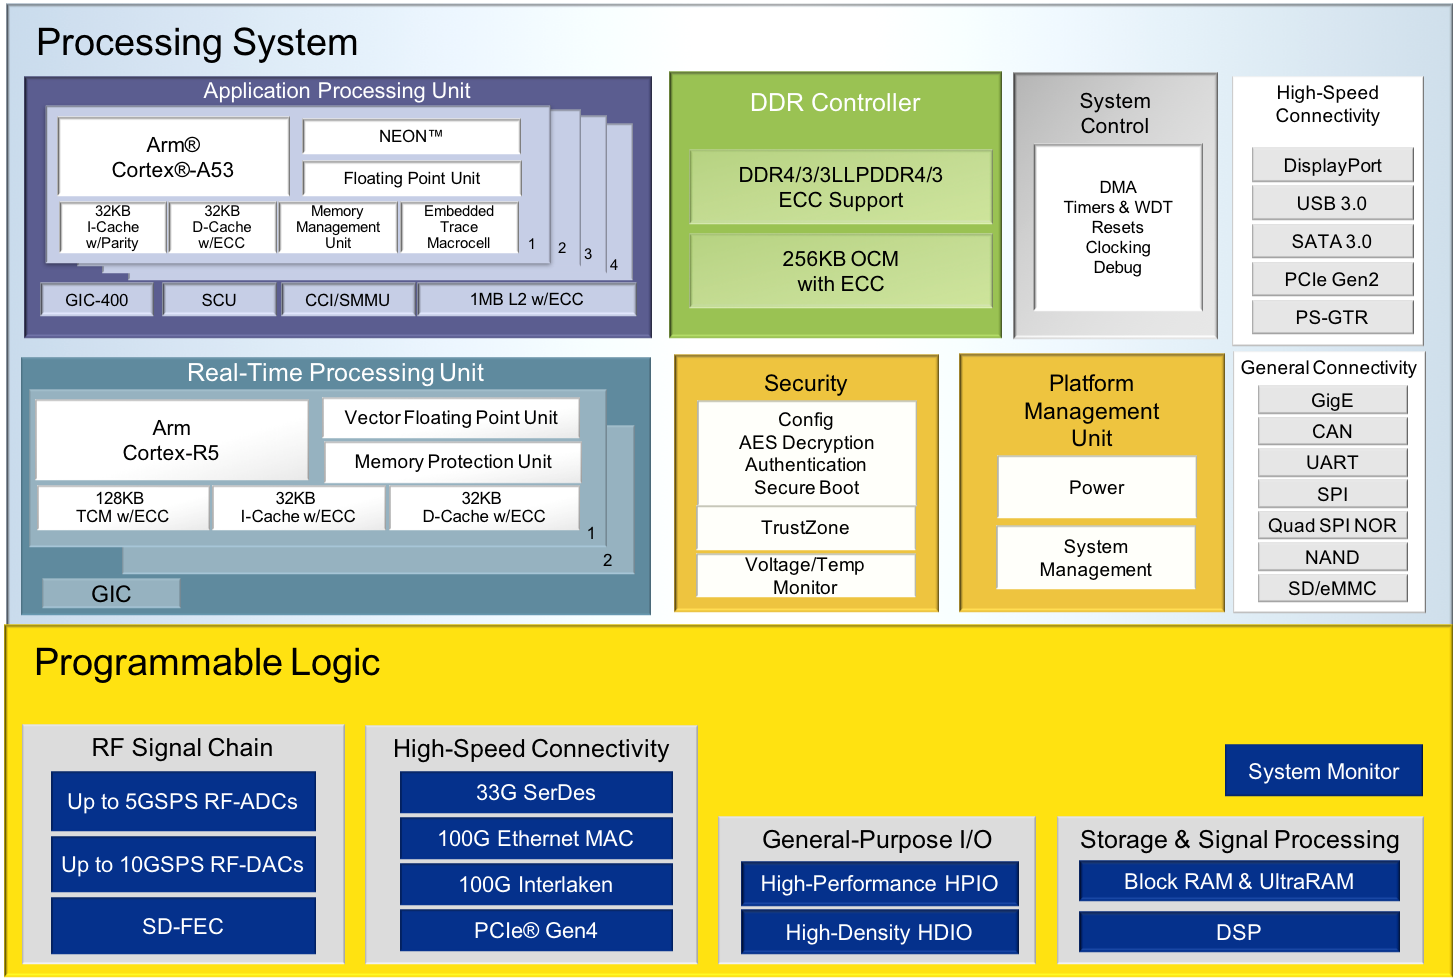
\includegraphics[width = 0.6\textwidth]{chap/03-work/img/rfsoc_blockdiagram}
	\caption{RFSoC block diagram}
	\label{fig:rfsoc}
\end{figure}

\subsection{Requirements}
\paragraph{Step size delay chip}
The necessary step size for the delay chips, when using 16 ADC@\SI{2}{\giga \sample \per \second} in time-interleaving mode, is: $\frac{\SI{2}{\giga \sample \per \second}}{16} = \SI{31}{\pico \second}$

\paragraph{Frequency}


\begin{figure}[H]
\centering
\tikzexternaldisable
\begin{tikztimingtable}
  TH1 & 1H 8L N(A1) 8L 16H \\
  TH2 & 2H 16L 15H \\
  TH3 & 3H 16L 14H \\
  TH4 & 4H 5L N(B1) 11L 13H \\
  \\
  TH5 & 5H 16L 12H \\
  TH6 & 6H 16L 11H \\
  TH7 & 7H 16L 10H \\
  TH8 & 8H 16L 9H \\
  \\
  TH9 & 9H 16L 8H \\
  TH10 & 10H 16L 7H \\
  TH11 & 11H 16L 6H \\
  TH12 & 12H 16L 5H \\
  \\
  TH13 & 13H 16L 4H \\
  TH14 & 14H 16L 3H \\
  TH15 & 15H 16L 2H \\
  TH16 & 16H 16L 1H \\
\extracode
 \tablerules
 \begin{pgfonlayer}{background}
 \draw [help lines, dashed] (A1) -- (B1);
 \end{pgfonlayer}
\end{tikztimingtable}
\tikzexternalenable
\caption{Track-And-Hold Timing diagram}
\label{fig:THA}
\end{figure}




\paragraph{Data Rate}
\paragraph{Visualization/GUI}
\newpage
\section{Design of the front-end card}
In this section, the design of the front-end card is covered.

\subsection{Sampling-Channel}
\paragraph{Track-And-Hold-Amplifier}
Explain why better than Sample-And-Hold-Amplifier.
\paragraph{Delay Chip NB6L295}
Dual Channel Programmable Delay Chip.

\begin{itemize}[noitemsep]
	\item Two individual variable delay channels
	\item Dual Delay: minimal delay \SI{3.2}{\nano \second}
	\item Total Delay Range: \SI{3.2}{\nano \second} to \SI{8.8}{\nano \second} per Delay Channel
	\item \SI{11}{\pico \second} Increments in 511 steps
	\item \SI{100}{\pico \second} Typical Rise and Fall Times
\end{itemize}

\subsection{Clocking}
On Xilinx CLK104 add-on board the LMX2594 is used to generate additional, high-frequency clocks for the ADCs/DACs. $\rightarrow$ reuse in front-end card
\begin{figure}[H]
	\centering
	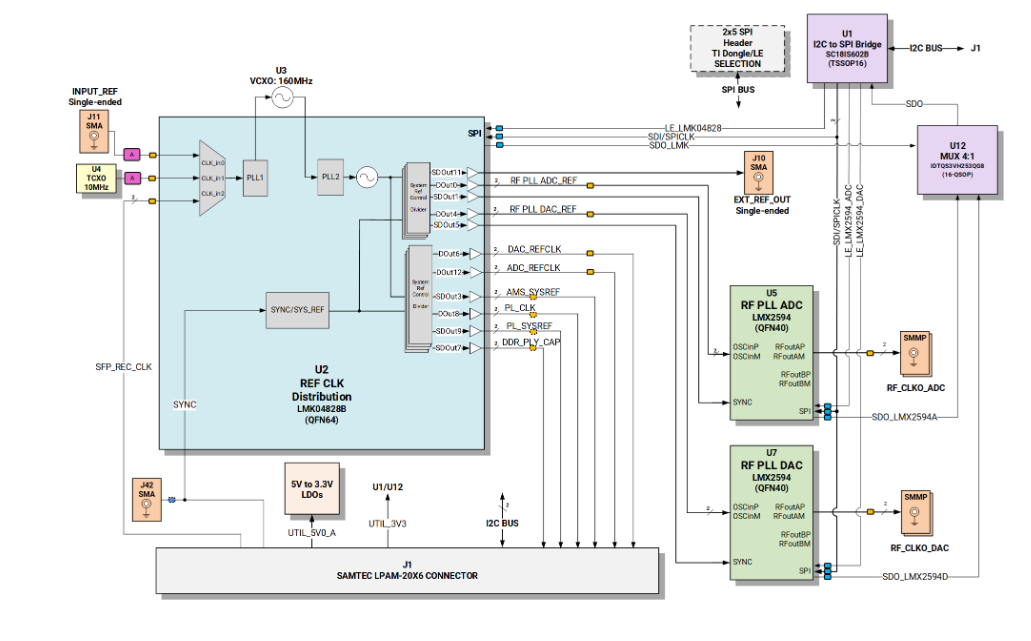
\includegraphics[width = 0.7\textwidth]{chap/03-work/img/clk104}
	\caption{CLK104 Add-on board clocking scheme}
	\label{fig:clk104}
\end{figure}

\begin{figure}[H]
	\centering
	\includegraphics[height = 0.3\textwidth, width = 0.55\textwidth]{chap/03-work/img/pll_tsMode.tikz}
	\caption{Clocking scheme on front-end card}
	\label{fig:clocking}
\end{figure}


\begin{figure}[H]
	\centering
	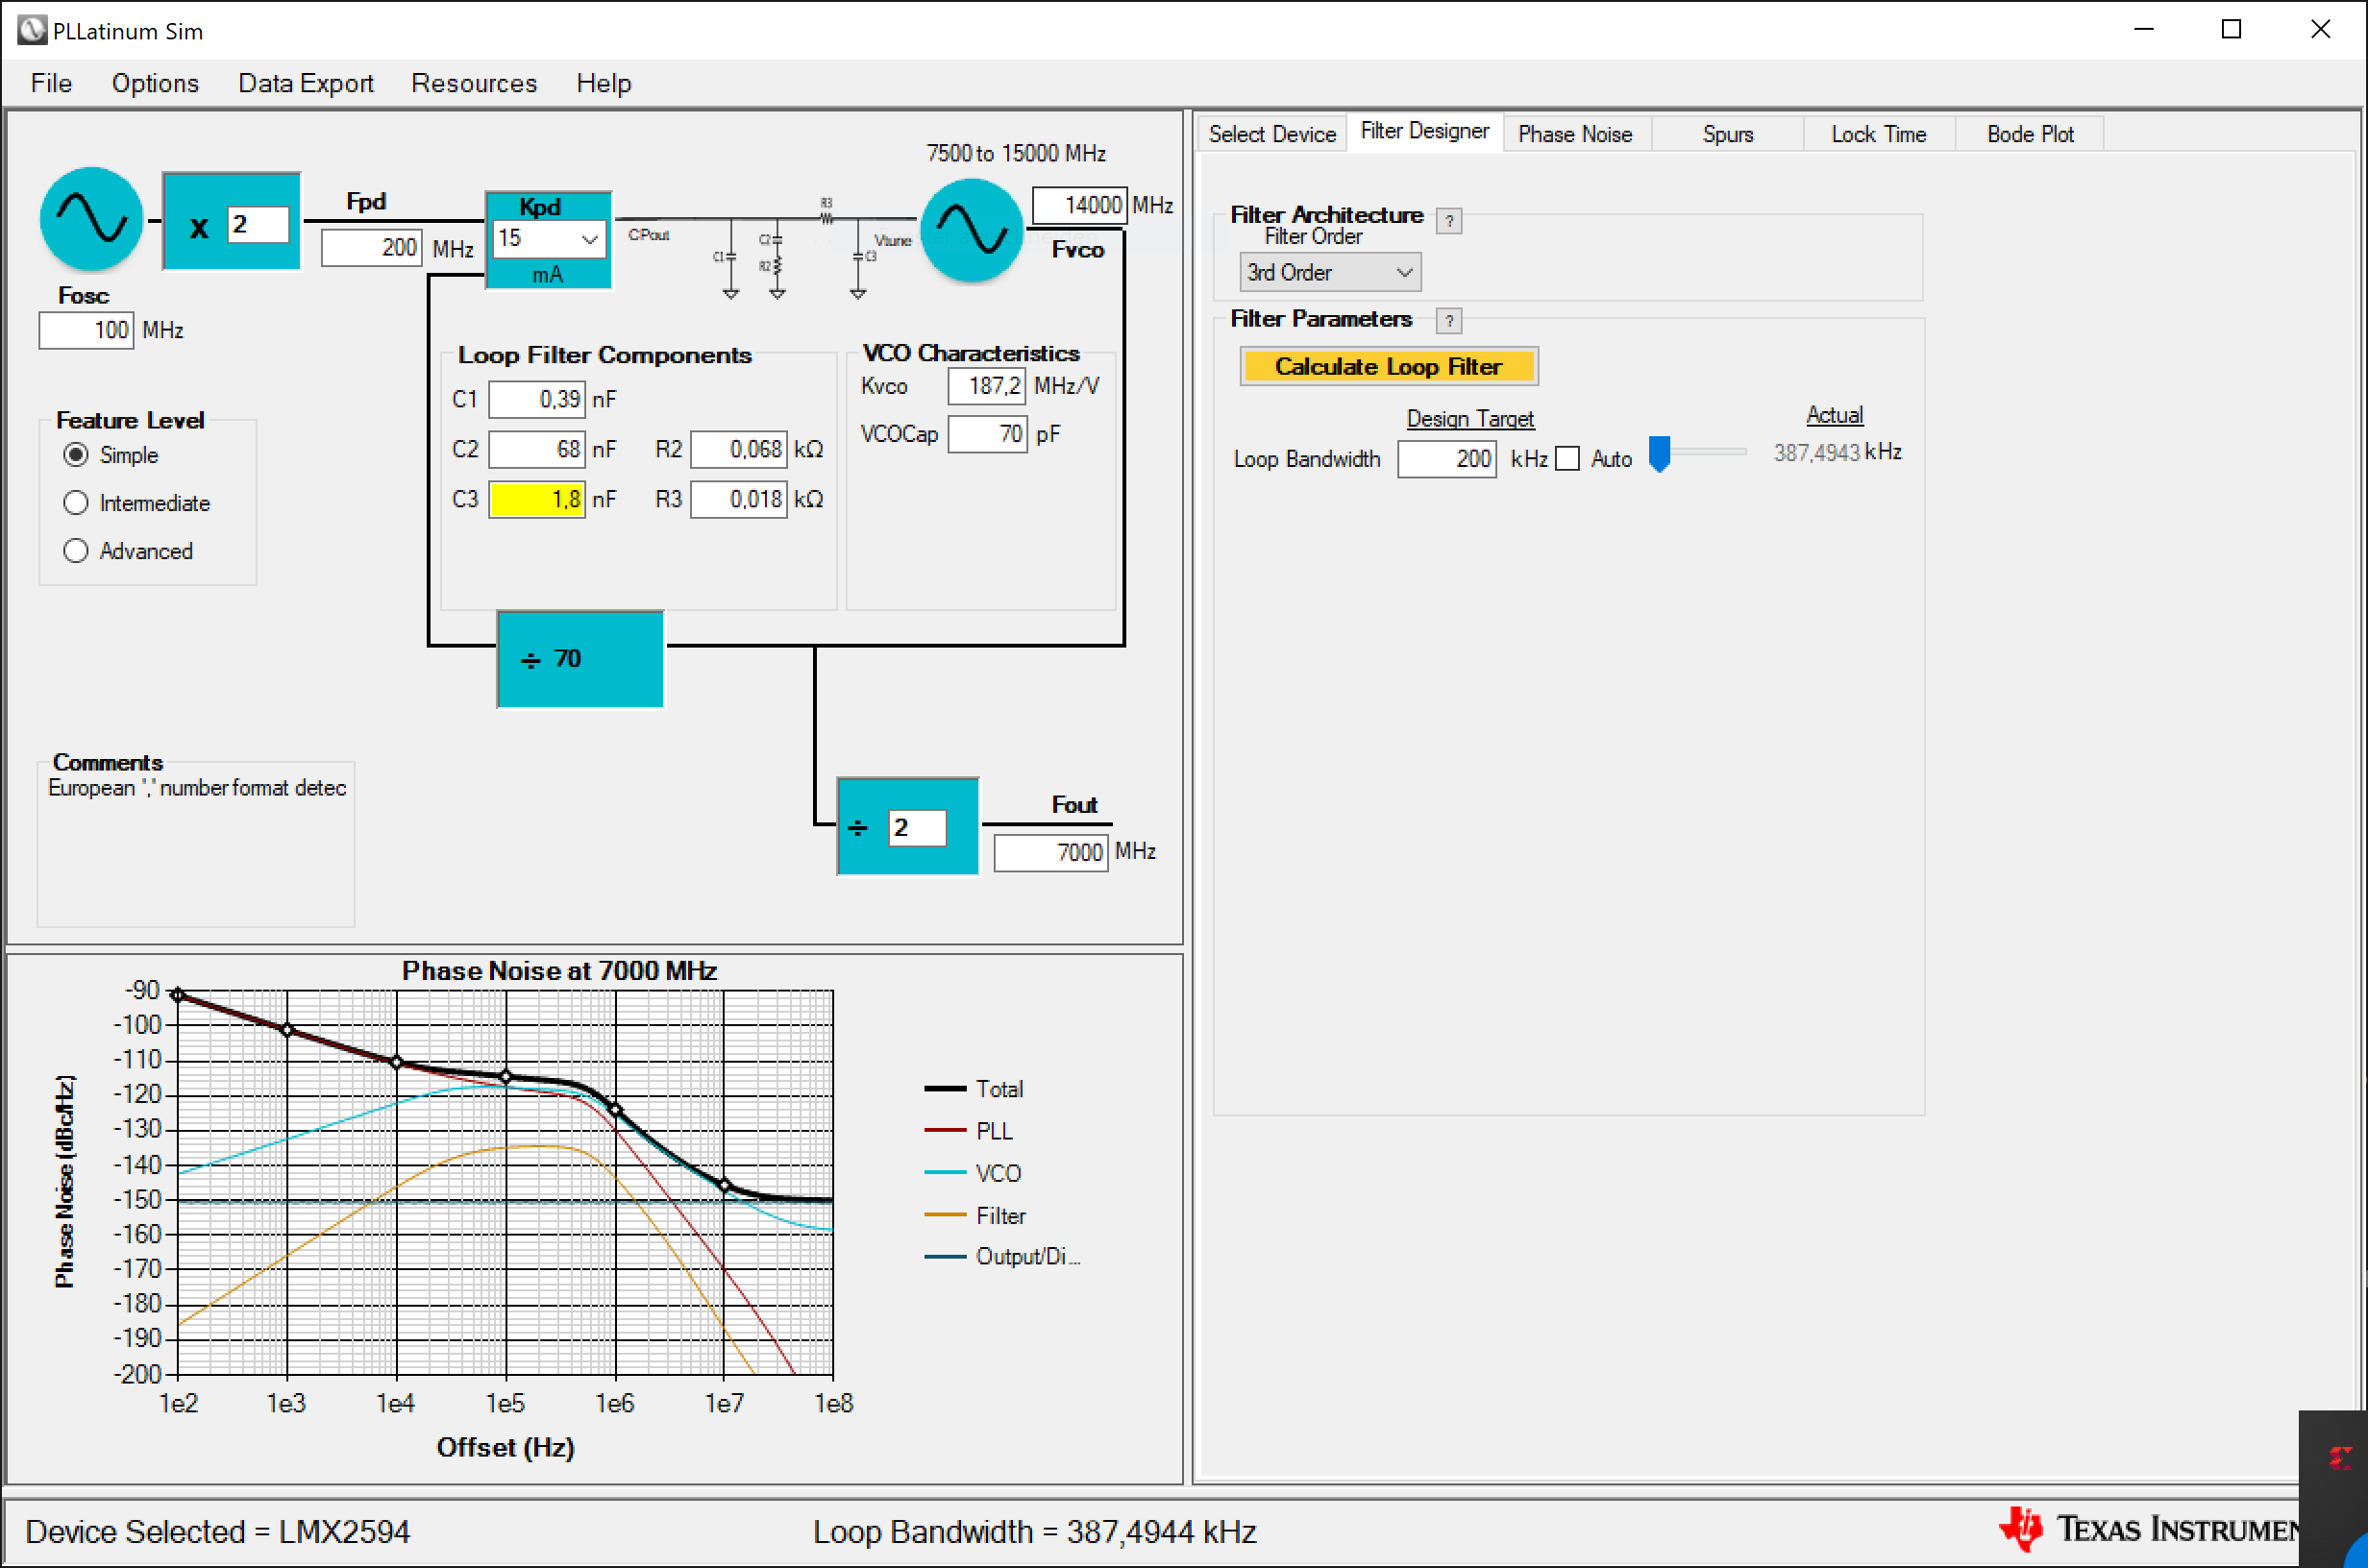
\includegraphics[width = 0.7\textwidth]{chap/03-work/img/pll.png}
	\caption{Placeholder}
	\label{fig:pll}
\end{figure}



\subsection{Power Supply}
For the Track-And-Hold amplifiers a new power supply unit -- the ADP1741 (Analog Devices) -- should be used. It is necessary to think about the amount of power supply chips needed. As a rule of thumb, the power supply should provide twice the maximum power needed by the components it drives. The power consumption/maximum current for the respective components on the THERESA board is listed in \autoref{tab:kapturecomp}. 
\begin{table}[tbh!]
	\caption{Power consumption of components on the board}
	\label{tab:kapturecomp}
	\begin{minipage}{\textwidth}
		\centering
		\begin{tabularx}{\textwidth}{XSSSSS}
			\toprule
			\textbf{Component} & \textbf{$V_{cc}$ (\SI{}{\volt})} & \textbf{$I_{max}$ (\SI{}{\ampere})} & \textbf{$P_{max}$ (\SI{}{\watt})} & $\#_{parts}$ & \textbf{$I_{tot}$}\footnote{for 16 ADCs} (\SI{}{\ampere})\\
				\midrule
			HMC5649 (T/H-Amplifier) 	& 2	  	& 0.221 	 & 0.442 & 16 & 3.536\\
									& -5  	& -0.242 & 1.21 &  & 3.872\\
			HMC856 (Delay) 			& -3.3	& 0.185 & -0.611 & 16 & 2.96\\
			HMC987LP5E (Fan-Out) 	& 3.3 	& 0.234\footnote{All Outputs and RF-Buffer} & 0.772 & 2 & 0.468\\
			LMC0480 (PLL) 			& 3.3 	& 0.590\footnote{All CLKs} & 1.947 & 1 & 0.590\\
			VCXO 					& 3.3 	& 0.03 & 0.198 & 1 & 0.03\\
			\bottomrule
		\end{tabularx}
	\end{minipage}
\end{table}

The maximal current which the ADP1741 can provide @\SI{2}{\volt} is \SI{2}{\ampere}. This means, with one Track-And-Hold amplifier requiring a maximal current of \SI{0.221}{\ampere}, one ADP1741 can handle four units according to the rule mentioned beforehand ($I_{max\_ADP1741} = \SI{2}{\ampere} > 2 * I_{tot}, I_{tot} = 4 \times \SI{0.221}{\ampere} =  \SI{0.884}{\ampere}$).



\newpage
\section{PCB-Layout}
\subsection{Substrate}
\subsection{Floor Planning}
\subsection{Transmission lines}

\begin{figure}[H]
	\centering
	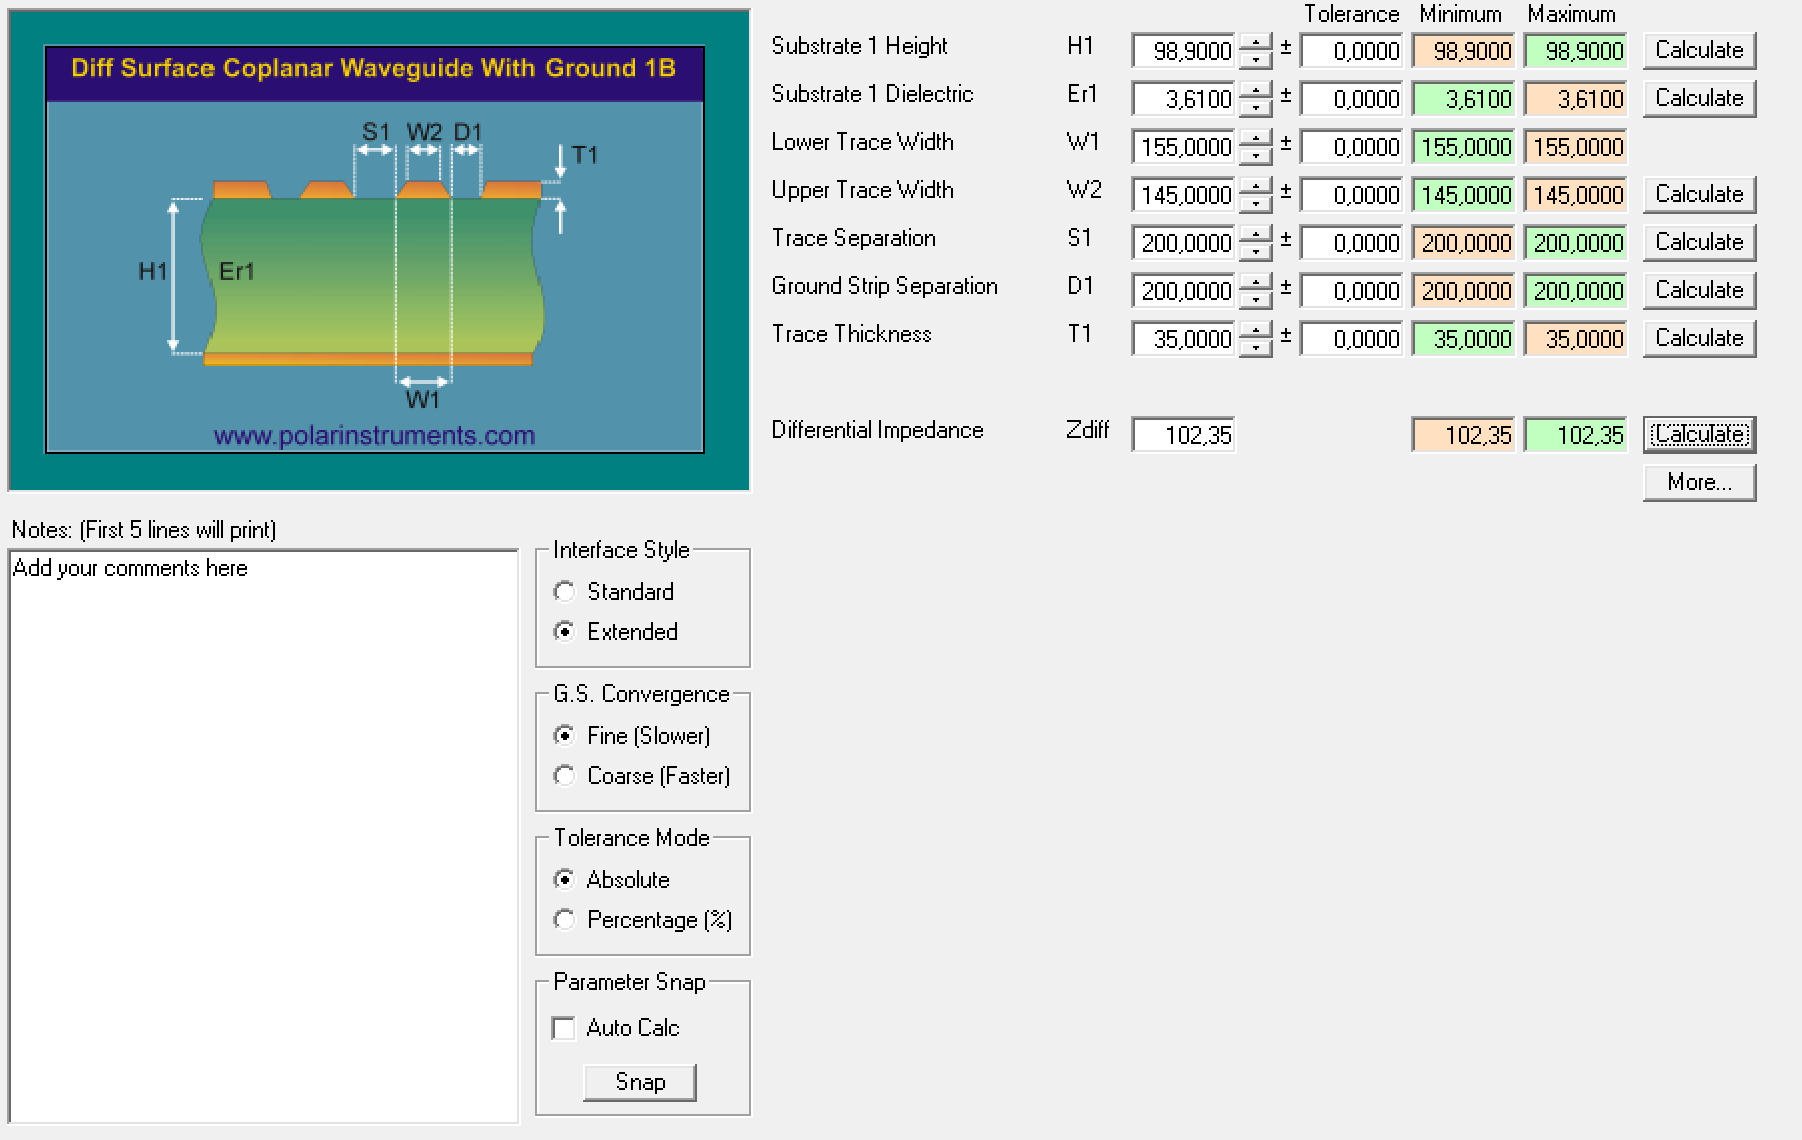
\includegraphics[width = 0.8\textwidth]{chap/03-work/img/polaris}
	\caption{Polaris Solver}
	\label{fig:polaris}
\end{figure}

\begin{figure}[H]
	\centering
	\includegraphics[width = \textwidth, height = 0.5\textwidth]{chap/03-work/img/megtron_diff_bottom_d1_vs_s1.tikz}
	\caption{Test Graph}
	\label{fig:megtron}
\end{figure}

  
\newpage
\section{Firmware}
\subsection{General Design}
\subsubsection{Firmware for Front-End Card}
\paragraph{Clocking}
\paragraph{SPI-Interface}
\subsubsection{Data Capture}
\begin{figure}[H]
	\centering
	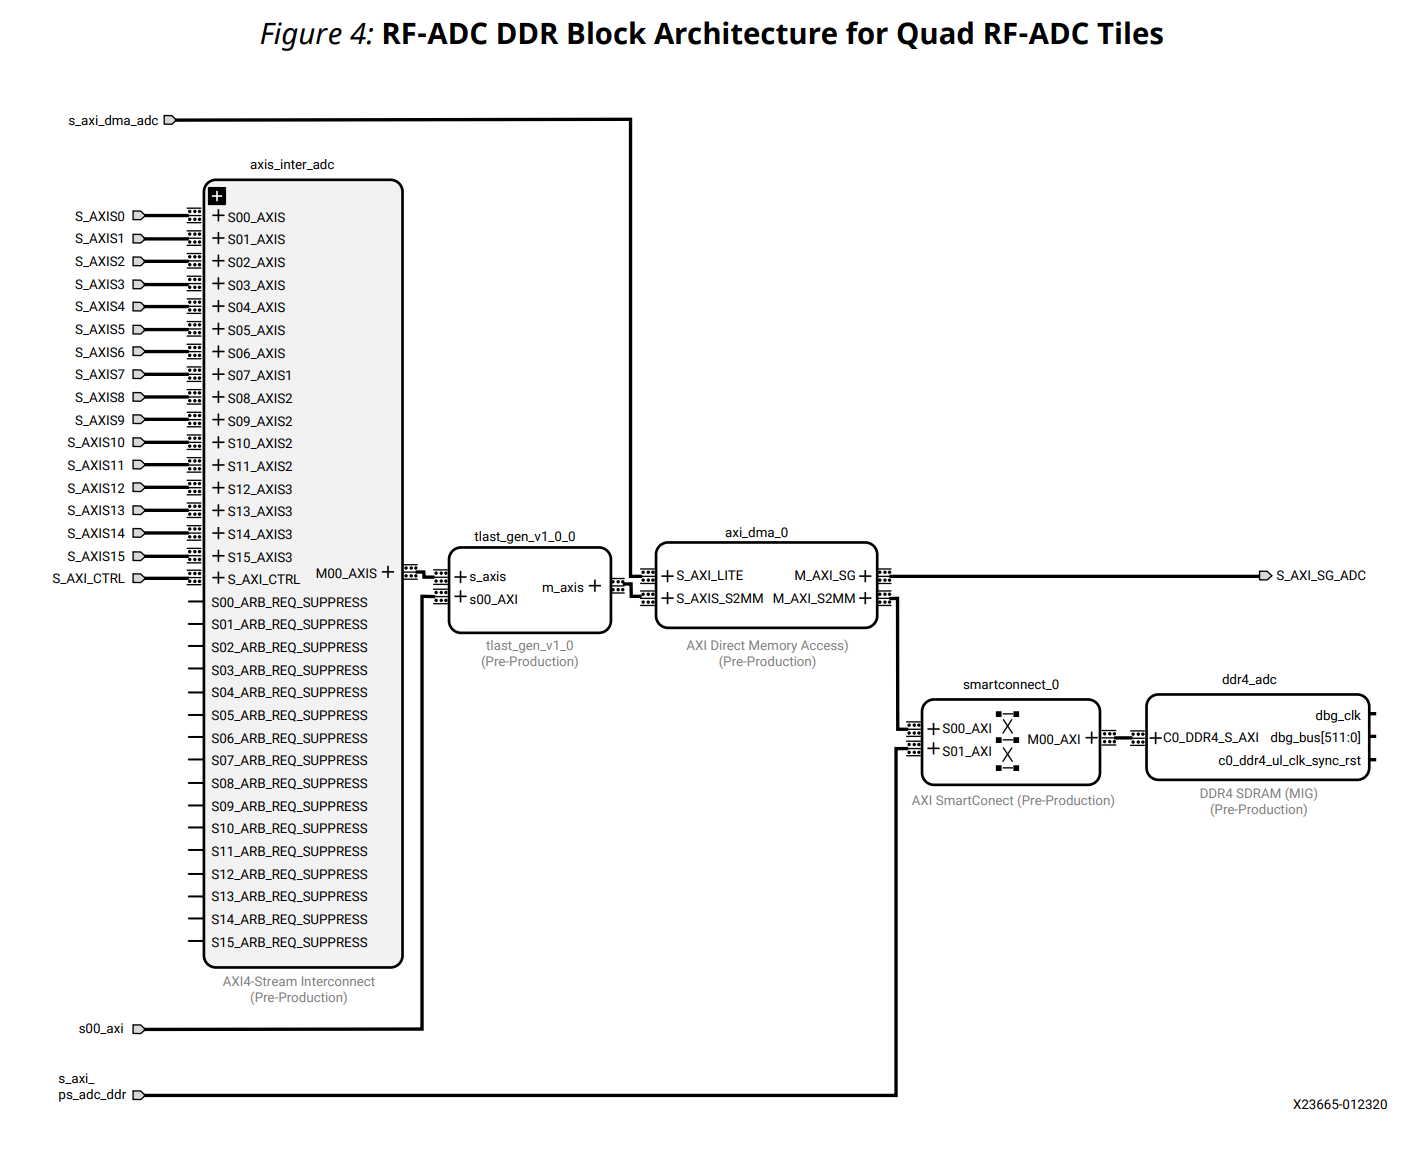
\includegraphics[width = 0.8\textwidth]{chap/03-work/img/adc_cap}
	\caption{Placeholder}
	\label{fig:adccap}
\end{figure}

\subsubsection{Visualization}





